

%\newcommand\DELTA{0.5}
\begin{figure}[!t]
\centering
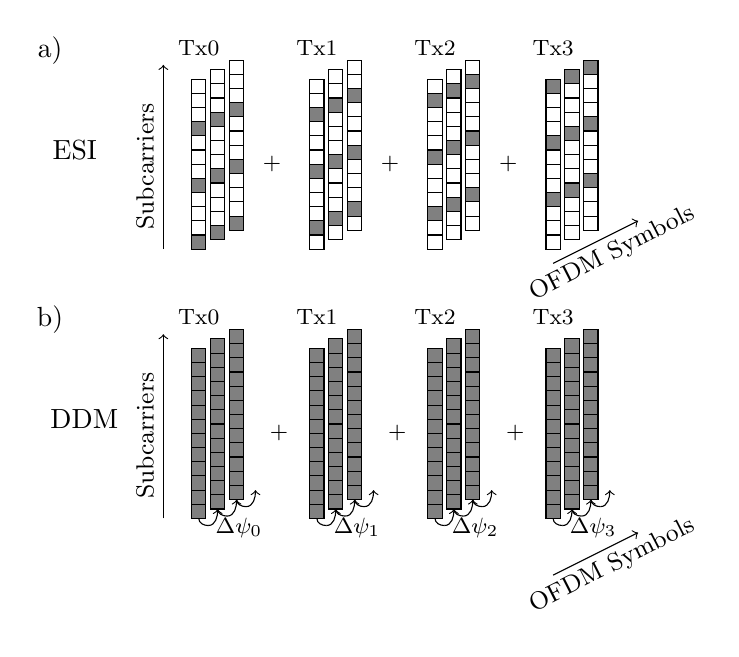
\begin{tikzpicture}[scale=0.6]
\def\d{2.2}%distance between two rows for ESI
\def\dr{2.5}%distance between two rows for RDMult
\def\a{0.3}%width of rectangle
\def\b{3.6}%height of rectangle
\def\hor_dist{5.7}%horizontal distance
\def\dx{0.4}%horizontal distance between symbols
\def\dy{0.2}%vertical distance between symbols

\begin{scope}[shift={(-3*\a,0)}]
%\node[right] at (-1,4.5) {a)};
% Draw axes

	\node at (-10*\a, \b + 2*\a) {a)}; 

	\draw[->] (-2*\a,0)  -- ++(0, \b+\a);
%    \draw [->,thick] (0,3.7) node (yaxis) [above] {}
%        |- (4.2,0) node (xaxis) [right] {};
%    \node[left] at (0,4-\DELTA/2) {\footnotesize $N_\text{c}-1$};    
%    \node[left] at (0,\DELTA/2) {\footnotesize $0$};    
%    \node[below] at (\DELTA/2,0 ) {\footnotesize $0$}; 
%    \node[below, text width=1cm, text centered] at (4 - \DELTA/2,0 ) {\footnotesize $N_\text{sym}-1$}; 
    \node[left, anchor=south, rotate=90] at (-2*\a,1.75) {\small Subcarriers};
%    \node[below] at (2,0) {OFDM symbols};
    

\foreach \inc in {0,...,2}
{	\draw[draw=black, fill=gray] (\inc*\dx,0+\inc*\dy) rectangle ++(\a, \a);
	\draw[draw=black, fill=white] (\inc*\dx,1*\a+\inc*\dy) rectangle ++(\a, \a);
	\draw[draw=black, fill=white] (\inc*\dx,2*\a+\inc*\dy) rectangle ++(\a, \a);
	\draw[draw=black, fill=white] (\inc*\dx,3*\a+\inc*\dy) rectangle ++(\a, \a);
	\draw[draw=black, fill=gray] (\inc*\dx,4*\a+\inc*\dy) rectangle ++(\a, \a);
	\draw[draw=black, fill=white] (\inc*\dx,5*\a+\inc*\dy) rectangle ++(\a, \a);
	\draw[draw=black, fill=white] (\inc*\dx,6*\a+\inc*\dy) rectangle ++(\a, \a);
	\draw[draw=black, fill=white] (\inc*\dx,7*\a+\inc*\dy) rectangle ++(\a, \a);
	\draw[draw=black, fill=gray] (\inc*\dx,8*\a+\inc*\dy) rectangle ++(\a, \a);
	\draw[draw=black, fill=white] (\inc*\dx,9*\a+\inc*\dy) rectangle ++(\a, \a);
	\draw[draw=black, fill=white] (\inc*\dx,10*\a+\inc*\dy) rectangle ++(\a, \a);
	\draw[draw=black, fill=white] (\inc*\dx,11*\a+\inc*\dy) rectangle ++(\a, \a);}

\node[left, anchor=north, rotate=27] at (5*\a ,10*\a) {\small $\hdots$};
	
	\node at (2*\a + 0.5*\d,0.5*\b) {\footnotesize $+$}; 
	\node[above] at (0.5*\a,\b+1*\a) {\footnotesize Tx0};
	

\foreach \inc in {0,...,2}
{	
  \draw[draw=black, fill=white] (\inc*\dx+\a + \d,0+\inc*\dy) rectangle ++(\a, \a);
	\draw[draw=black, fill=gray] (\inc*\dx+\a + \d,1*\a+\inc*\dy) rectangle ++(\a, \a);
	\draw[draw=black, fill=white] (\inc*\dx+\a + \d,2*\a+\inc*\dy) rectangle ++(\a, \a);
	\draw[draw=black, fill=white] (\inc*\dx+\a + \d,3*\a+\inc*\dy) rectangle ++(\a, \a);
	\draw[draw=black, fill=white] (\inc*\dx+\a + \d,4*\a+\inc*\dy) rectangle ++(\a, \a);
	\draw[draw=black, fill=gray] (\inc*\dx+\a + \d,5*\a+\inc*\dy) rectangle ++(\a, \a);
	\draw[draw=black, fill=white] (\inc*\dx+\a + \d,6*\a+\inc*\dy) rectangle ++(\a, \a);
	\draw[draw=black, fill=white] (\inc*\dx+\a + \d,7*\a+\inc*\dy) rectangle ++(\a, \a);
	\draw[draw=black, fill=white] (\inc*\dx+\a + \d,8*\a+\inc*\dy) rectangle ++(\a, \a);
	\draw[draw=black, fill=gray] (\inc*\dx+\a + \d,9*\a+\inc*\dy) rectangle ++(\a, \a);
	\draw[draw=black, fill=white] (\inc*\dx+\a + \d,10*\a+\inc*\dy) rectangle ++(\a, \a);
	\draw[draw=black, fill=white] (\inc*\dx+\a + \d,11*\a+\inc*\dy) rectangle ++(\a, \a);}
	
	\node[left, anchor=north, rotate=27] at (5*\a +\a + \d,10*\a) {\small $\hdots$};
	
%	\draw[draw=black, fill=gray] (\a + \d,\a) rectangle ++(\a, \a);
%	\draw[draw=black, fill=gray] (\a + \d,5*\a) rectangle ++(\a, \a);	
%	\draw[draw=black, fill=gray] (\a + \d,9*\a) rectangle ++(\a, \a);
	
	\node at (3*\a + 1.5*\d,0.5*\b) {\footnotesize $+$}; 
	\node[above] at (1.5*\a+\d,\b+1*\a) {\footnotesize Tx1};
	
\foreach \inc in {0,...,2}
{	\draw[draw=black, fill=white] (\inc*\dx+2*\a + 2*\d,0+\inc*\dy) rectangle ++(\a, \a);
	\draw[draw=black, fill=white] (\inc*\dx+2*\a + 2*\d,1*\a+\inc*\dy) rectangle ++(\a, \a);
	\draw[draw=black, fill=gray] (\inc*\dx+2*\a + 2*\d,2*\a+\inc*\dy) rectangle ++(\a, \a);
	\draw[draw=black, fill=white] (\inc*\dx+2*\a + 2*\d,3*\a+\inc*\dy) rectangle ++(\a, \a);
	\draw[draw=black, fill=white] (\inc*\dx+2*\a + 2*\d,4*\a+\inc*\dy) rectangle ++(\a, \a);
	\draw[draw=black, fill=white] (\inc*\dx+2*\a + 2*\d,5*\a+\inc*\dy) rectangle ++(\a, \a);
	\draw[draw=black, fill=gray] (\inc*\dx+2*\a + 2*\d,6*\a+\inc*\dy) rectangle ++(\a, \a);
	\draw[draw=black, fill=white] (\inc*\dx+2*\a + 2*\d,7*\a+\inc*\dy) rectangle ++(\a, \a);
	\draw[draw=black, fill=white] (\inc*\dx+2*\a + 2*\d,8*\a+\inc*\dy) rectangle ++(\a, \a);
	\draw[draw=black, fill=white] (\inc*\dx+2*\a + 2*\d,9*\a+\inc*\dy) rectangle ++(\a, \a);
	\draw[draw=black, fill=gray] (\inc*\dx+2*\a + 2*\d,10*\a+\inc*\dy) rectangle ++(\a, \a);
	\draw[draw=black, fill=white] (\inc*\dx+2*\a + 2*\d,11*\a+\inc*\dy) rectangle ++(\a, \a);}
	
	\node[left, anchor=north, rotate=27] at (5*\a + 2*\a + 2*\d,10*\a) {\small $\hdots$};
	
%	\draw[draw=black, fill=gray] (2*\a + 2*\d,2*\a) rectangle ++(\a, \a);
%	\draw[draw=black, fill=gray] (2*\a + 2*\d,6*\a) rectangle ++(\a, \a);	
%	\draw[draw=black, fill=gray] (2*\a + 2*\d,10*\a) rectangle ++(\a, \a);
	
	\node at (4*\a + 2.5*\d,0.5*\b) {\footnotesize $+$}; 
	\node[above] at (2.5*\a+2*\d,\b+1*\a) {\footnotesize Tx2};
	
\foreach \inc in {0,...,2}
{	\draw[draw=black, fill=white] (\inc*\dx+3*\a + 3*\d,0+\inc*\dy) rectangle ++(\a, \a);
	\draw[draw=black, fill=white] (\inc*\dx+3*\a + 3*\d,1*\a+\inc*\dy) rectangle ++(\a, \a);
	\draw[draw=black, fill=white] (\inc*\dx+3*\a + 3*\d,2*\a+\inc*\dy) rectangle ++(\a, \a);
	\draw[draw=black, fill=gray] (\inc*\dx+3*\a + 3*\d,3*\a+\inc*\dy) rectangle ++(\a, \a);
	\draw[draw=black, fill=white] (\inc*\dx+3*\a + 3*\d,4*\a+\inc*\dy) rectangle ++(\a, \a);
	\draw[draw=black, fill=white] (\inc*\dx+3*\a + 3*\d,5*\a+\inc*\dy) rectangle ++(\a, \a);
	\draw[draw=black, fill=white] (\inc*\dx+3*\a + 3*\d,6*\a+\inc*\dy) rectangle ++(\a, \a);
	\draw[draw=black, fill=gray] (\inc*\dx+3*\a + 3*\d,7*\a+\inc*\dy) rectangle ++(\a, \a);
	\draw[draw=black, fill=white] (\inc*\dx+3*\a + 3*\d,8*\a+\inc*\dy) rectangle ++(\a, \a);
	\draw[draw=black, fill=white] (\inc*\dx+3*\a + 3*\d,9*\a+\inc*\dy) rectangle ++(\a, \a);
	\draw[draw=black, fill=white] (\inc*\dx+3*\a + 3*\d,10*\a+\inc*\dy) rectangle ++(\a, \a);
	\draw[draw=black, fill=gray] (\inc*\dx+3*\a + 3*\d,11*\a+\inc*\dy) rectangle ++(\a, \a);}
	
	\node[left, anchor=north, rotate=27] at (5*\a+3*\a + 3*\d ,10*\a) {\small $\hdots$};
	
	\draw[->] (\a/2+3*\a + 3*\d,-\a)  -- ++(6*\a, 3*\a);
	\node[left, anchor=north, rotate=27] at (7*\a + 3*\d,1*\a) {\small OFDM Symbols};
	
	\node[above] at (3.5*\a+3*\d,\b+1*\a) {\footnotesize Tx3};
	%\node[above] at (2*\a+1.5*\d,\b+3*\a) {ESI};
	\node[left] at (-6*\a,0.5*\b+1*\a) {ESI};
\end{scope}

  
  \begin{scope}[shift={(-3*\a,-\hor_dist)}]

	\node at (-10*\a, \b + 2*\a) {b)}; 
	\node[left] at (-4.5*\a,0.5*\b+1*\a) {DDM};

	\draw[->] (-2*\a,0)  -- ++(0, \b+\a);
    \node[left, anchor=south, rotate=90] at (-2*\a,1.75) {\small Subcarriers};
    
\foreach \inc in {0,...,2}
{	\draw[draw=black, fill=gray] (\inc*\dx+0,0+\inc*\dy) rectangle ++(\a, \a);
	\draw[draw=black, fill=gray] (\inc*\dx+0,1*\a+\inc*\dy) rectangle ++(\a, \a);
	\draw[draw=black, fill=gray] (\inc*\dx+0,2*\a+\inc*\dy) rectangle ++(\a, \a);
	\draw[draw=black, fill=gray] (\inc*\dx+0,3*\a+\inc*\dy) rectangle ++(\a, \a);
	\draw[draw=black, fill=gray] (\inc*\dx+0,4*\a+\inc*\dy) rectangle ++(\a, \a);
	\draw[draw=black, fill=gray] (\inc*\dx+0,5*\a+\inc*\dy) rectangle ++(\a, \a);
	\draw[draw=black, fill=gray] (\inc*\dx+0,6*\a+\inc*\dy) rectangle ++(\a, \a);
	\draw[draw=black, fill=gray] (\inc*\dx+0,7*\a+\inc*\dy) rectangle ++(\a, \a);
	\draw[draw=black, fill=gray] (\inc*\dx+0,8*\a+\inc*\dy) rectangle ++(\a, \a);
	\draw[draw=black, fill=gray] (\inc*\dx+0,9*\a+\inc*\dy) rectangle ++(\a, \a);
	\draw[draw=black, fill=gray] (\inc*\dx+0,10*\a+\inc*\dy) rectangle ++(\a, \a);
	\draw[draw=black, fill=gray] (\inc*\dx+0,11*\a+\inc*\dy) rectangle ++(\a, \a);}
	
		\node[left, anchor=north, rotate=27] at (5*\a ,10*\a) {\small $\hdots$};
		
		
	
	\draw [-] (0.5*\a, 0) to [out=270,in=180] (0.5*\a+0.5*\dx, -0.5*\a);
	\draw [->] (0.5*\a+0.5*\dx, -0.5*\a) to [out=0,in=270] (0.5*\a+\dx, 0+\dy);
	\draw [-] (0.5*\a+\dx, 0+\dy) to [out=270,in=180] (0.5*\a+0.5*\dx+\dx, -0.5*\a+\dy);
	\draw [->] (0.5*\a+0.5*\dx+\dx, -0.5*\a+\dy) to [out=0,in=270] (0.5*\a+\dx+\dx, 0+\dy+\dy);
	\draw [-] (0.5*\a+2*\dx, 0+2*\dy) to [out=270,in=180] (0.5*\a+0.5*\dx+2*\dx, -0.5*\a+2*\dy);
	\draw [->] (0.5*\a+0.5*\dx+2*\dx, -0.5*\a+2*\dy) to [out=0,in=270] (0.5*\a+\dx+2*\dx, 0+\dy+2*\dy);
	
	\node[right] at (1*\a ,-0.7*\a) {\footnotesize $\Delta \psi_0$}; 
	
	\node at (2*\a + 0.5*\dr,0.5*\b) {\footnotesize $+$}; 
	\node[above] at (0.5*\a,\b+1*\a) {\footnotesize Tx0};
	

\end{scope}

\begin{scope}[shift={(\dr-3*\a,-\hor_dist)}]
    
\foreach \inc in {0,...,2}
{	\draw[draw=black, fill=gray] (\inc*\dx+0,0+\inc*\dy) rectangle ++(\a, \a);
	\draw[draw=black, fill=gray] (\inc*\dx+0,1*\a+\inc*\dy) rectangle ++(\a, \a);
	\draw[draw=black, fill=gray] (\inc*\dx+0,2*\a+\inc*\dy) rectangle ++(\a, \a);
	\draw[draw=black, fill=gray] (\inc*\dx+0,3*\a+\inc*\dy) rectangle ++(\a, \a);
	\draw[draw=black, fill=gray] (\inc*\dx+0,4*\a+\inc*\dy) rectangle ++(\a, \a);
	\draw[draw=black, fill=gray] (\inc*\dx+0,5*\a+\inc*\dy) rectangle ++(\a, \a);
	\draw[draw=black, fill=gray] (\inc*\dx+0,6*\a+\inc*\dy) rectangle ++(\a, \a);
	\draw[draw=black, fill=gray] (\inc*\dx+0,7*\a+\inc*\dy) rectangle ++(\a, \a);
	\draw[draw=black, fill=gray] (\inc*\dx+0,8*\a+\inc*\dy) rectangle ++(\a, \a);
	\draw[draw=black, fill=gray] (\inc*\dx+0,9*\a+\inc*\dy) rectangle ++(\a, \a);
	\draw[draw=black, fill=gray] (\inc*\dx+0,10*\a+\inc*\dy) rectangle ++(\a, \a);
	\draw[draw=black, fill=gray] (\inc*\dx+0,11*\a+\inc*\dy) rectangle ++(\a, \a);}
	
		\node[left, anchor=north, rotate=27] at (5*\a ,10*\a) {\small $\hdots$};
		
		
	\draw [-] (0.5*\a, 0) to [out=270,in=180] (0.5*\a+0.5*\dx, -0.5*\a);
	\draw [->] (0.5*\a+0.5*\dx, -0.5*\a) to [out=0,in=270] (0.5*\a+\dx, 0+\dy);
	\draw [-] (0.5*\a+\dx, 0+\dy) to [out=270,in=180] (0.5*\a+0.5*\dx+\dx, -0.5*\a+\dy);
	\draw [->] (0.5*\a+0.5*\dx+\dx, -0.5*\a+\dy) to [out=0,in=270] (0.5*\a+\dx+\dx, 0+\dy+\dy);
	\draw [-] (0.5*\a+2*\dx, 0+2*\dy) to [out=270,in=180] (0.5*\a+0.5*\dx+2*\dx, -0.5*\a+2*\dy);
	\draw [->] (0.5*\a+0.5*\dx+2*\dx, -0.5*\a+2*\dy) to [out=0,in=270] (0.5*\a+\dx+2*\dx, 0+\dy+2*\dy);
	
	\node[right] at (1*\a ,-0.7*\a) {\footnotesize $\Delta \psi_1$}; 
	
	\node at (2*\a + 0.5*\dr,0.5*\b) {\footnotesize $+$}; 
	\node[above] at (0.5*\a,\b+1*\a) {\footnotesize Tx1};
	

\end{scope}

\begin{scope}[shift={(2*\dr-3*\a,-\hor_dist)}]
    
\foreach \inc in {0,...,2}
{	\draw[draw=black, fill=gray] (\inc*\dx+0,0+\inc*\dy) rectangle ++(\a, \a);
	\draw[draw=black, fill=gray] (\inc*\dx+0,1*\a+\inc*\dy) rectangle ++(\a, \a);
	\draw[draw=black, fill=gray] (\inc*\dx+0,2*\a+\inc*\dy) rectangle ++(\a, \a);
	\draw[draw=black, fill=gray] (\inc*\dx+0,3*\a+\inc*\dy) rectangle ++(\a, \a);
	\draw[draw=black, fill=gray] (\inc*\dx+0,4*\a+\inc*\dy) rectangle ++(\a, \a);
	\draw[draw=black, fill=gray] (\inc*\dx+0,5*\a+\inc*\dy) rectangle ++(\a, \a);
	\draw[draw=black, fill=gray] (\inc*\dx+0,6*\a+\inc*\dy) rectangle ++(\a, \a);
	\draw[draw=black, fill=gray] (\inc*\dx+0,7*\a+\inc*\dy) rectangle ++(\a, \a);
	\draw[draw=black, fill=gray] (\inc*\dx+0,8*\a+\inc*\dy) rectangle ++(\a, \a);
	\draw[draw=black, fill=gray] (\inc*\dx+0,9*\a+\inc*\dy) rectangle ++(\a, \a);
	\draw[draw=black, fill=gray] (\inc*\dx+0,10*\a+\inc*\dy) rectangle ++(\a, \a);
	\draw[draw=black, fill=gray] (\inc*\dx+0,11*\a+\inc*\dy) rectangle ++(\a, \a);}
	
		\node[left, anchor=north, rotate=27] at (5*\a ,10*\a) {\small $\hdots$};
	
	\draw [-] (0.5*\a, 0) to [out=270,in=180] (0.5*\a+0.5*\dx, -0.5*\a);
	\draw [->] (0.5*\a+0.5*\dx, -0.5*\a) to [out=0,in=270] (0.5*\a+\dx, 0+\dy);
	\draw [-] (0.5*\a+\dx, 0+\dy) to [out=270,in=180] (0.5*\a+0.5*\dx+\dx, -0.5*\a+\dy);
	\draw [->] (0.5*\a+0.5*\dx+\dx, -0.5*\a+\dy) to [out=0,in=270] (0.5*\a+\dx+\dx, 0+\dy+\dy);
	\draw [-] (0.5*\a+2*\dx, 0+2*\dy) to [out=270,in=180] (0.5*\a+0.5*\dx+2*\dx, -0.5*\a+2*\dy);
	\draw [->] (0.5*\a+0.5*\dx+2*\dx, -0.5*\a+2*\dy) to [out=0,in=270] (0.5*\a+\dx+2*\dx, 0+\dy+2*\dy);
	
	\node[right] at (1*\a ,-0.7*\a) {\footnotesize $\Delta \psi_2$}; 
	
	\node at (2*\a + 0.5*\dr,0.5*\b) {\footnotesize $+$}; 
	\node[above] at (0.5*\a,\b+1*\a) {\footnotesize Tx2};
	

\end{scope}
\begin{scope}[shift={(3*\dr-3*\a,-\hor_dist)}]
    
\foreach \inc in {0,...,2}
{	\draw[draw=black, fill=gray] (\inc*\dx+0,0+\inc*\dy) rectangle ++(\a, \a);
	\draw[draw=black, fill=gray] (\inc*\dx+0,1*\a+\inc*\dy) rectangle ++(\a, \a);
	\draw[draw=black, fill=gray] (\inc*\dx+0,2*\a+\inc*\dy) rectangle ++(\a, \a);
	\draw[draw=black, fill=gray] (\inc*\dx+0,3*\a+\inc*\dy) rectangle ++(\a, \a);
	\draw[draw=black, fill=gray] (\inc*\dx+0,4*\a+\inc*\dy) rectangle ++(\a, \a);
	\draw[draw=black, fill=gray] (\inc*\dx+0,5*\a+\inc*\dy) rectangle ++(\a, \a);
	\draw[draw=black, fill=gray] (\inc*\dx+0,6*\a+\inc*\dy) rectangle ++(\a, \a);
	\draw[draw=black, fill=gray] (\inc*\dx+0,7*\a+\inc*\dy) rectangle ++(\a, \a);
	\draw[draw=black, fill=gray] (\inc*\dx+0,8*\a+\inc*\dy) rectangle ++(\a, \a);
	\draw[draw=black, fill=gray] (\inc*\dx+0,9*\a+\inc*\dy) rectangle ++(\a, \a);
	\draw[draw=black, fill=gray] (\inc*\dx+0,10*\a+\inc*\dy) rectangle ++(\a, \a);
	\draw[draw=black, fill=gray] (\inc*\dx+0,11*\a+\inc*\dy) rectangle ++(\a, \a);}
	

		\draw [-] (0.5*\a, 0) to [out=270,in=180] (0.5*\a+0.5*\dx, -0.5*\a);
	\draw [->] (0.5*\a+0.5*\dx, -0.5*\a) to [out=0,in=270] (0.5*\a+\dx, 0+\dy);
	\draw [-] (0.5*\a+\dx, 0+\dy) to [out=270,in=180] (0.5*\a+0.5*\dx+\dx, -0.5*\a+\dy);
	\draw [->] (0.5*\a+0.5*\dx+\dx, -0.5*\a+\dy) to [out=0,in=270] (0.5*\a+\dx+\dx, 0+\dy+\dy);
	\draw [-] (0.5*\a+2*\dx, 0+2*\dy) to [out=270,in=180] (0.5*\a+0.5*\dx+2*\dx, -0.5*\a+2*\dy);
	\draw [->] (0.5*\a+0.5*\dx+2*\dx, -0.5*\a+2*\dy) to [out=0,in=270] (0.5*\a+\dx+2*\dx, 0+\dy+2*\dy);
	
	\node[right] at (1*\a ,-0.7*\a) {\footnotesize $\Delta \psi_3$}; 
	
	
	\node[left, anchor=north, rotate=27] at (5*\a ,10*\a) {\small $\hdots$};
	
	\node[above] at (0.5*\a,\b+1*\a) {\footnotesize Tx3};
	
		\draw[->] (\a/2+3*\a + 3*\d-3*\dr,-4*\a)  -- ++(6*\a, 3*\a);
	\node[left, anchor=north, rotate=27] at (7*\a + 3*\d-3*\dr,-2*\a) {\small OFDM Symbols};

\end{scope}



\end{tikzpicture}
 \caption{a) Schematic visualization of the subcarrier allocation for ESI for the special case of 4 Tx antennas. Only every 4th subcarrier is active (gray blocks) for each Tx antenna. b) Sketch of the principle of DDM with unique phase shifts $\Delta \psi_k$ from OFDM symbol to OFDM symbol that shifts the received signals along the velocity axis. $k$ denotes the Tx antenna index. }
\label{fig_MIMO_spectral_interleaving}
\end{figure}



